\documentclass[11pt,letterpaper]{article}
\usepackage[margin=0.78in]{geometry}
\usepackage{amsmath,amssymb,booktabs,tabularx,array,graphicx,xcolor,fancyhdr,hyperref}
\definecolor{teal}{HTML}{246E80}
\hypersetup{colorlinks=true,urlcolor=teal,linkcolor=teal}
\pagestyle{fancy}\fancyhf{}\lhead{\small WikiFlow / Initial ML Solution}\rhead{\small 22 October 2026}\cfoot{\small\thepage}
\setlength{\headheight}{14pt}\setlength{\emergencystretch}{2em}
\setlength{\parindent}{0pt}\setlength{\parskip}{7pt}
\renewcommand{\arraystretch}{1.17}
\newcommand{\sect}[1]{\vspace{4pt}{\large\bfseries\color{teal}#1}\par}
\newcommand{\src}[1]{{\small\textit{Evidence: #1}}}
\begin{document}
{\LARGE\bfseries WikiFlow}\par
{\Large A monthly shortlist for AI-topic article review}\par
{\large Initial ML Solution -- binary event ranking}\par
Team INFO $\cdot$ 10-718 Machine Learning in Practice\par
We study whether learned rankings help volunteers identify future traffic surges among currently cold, lightly edited AI-maintenance articles. The report compares fixed traffic rules with linear, boosted-tree and pairwise ranking models on a common chronological backtest.

\sect{1. Task, population and feedback response}
WikiFlow ranks Wikipedia articles for volunteers to review before a possible increase in internal navigation. The unit is an \textbf{article--month}. The population is a fixed WikiProject Artificial Intelligence maintenance catalogue of 1,187 canonical articles, including people and works. It is not a census of all AI content. At each monthly decision, eligibility restricts the list to currently cold articles with sufficiently complete history and little recent substantial editing.

The operational objective is to reduce the number and proportion of future surge articles that lack substantial editing beforehand, by directing limited volunteer attention to them. The offline label is a traffic event, not proof that an article needs an edit or that an intervention improves quality. NDCG@50 is an offline ranking proxy for allocating that attention; a deployment pilot would additionally measure timely edits and useful reviews per volunteer-hour. The working budget is \textbf{50 articles per month}; it has not been validated against actual volunteer capacity.

The prior feedback, verified on October 20, marked \textbf{metric choice} and \textbf{baseline results} as Needs Work. This report responds by defining the population, budget and metric aggregation explicitly, including both Volume and Momentum under exactly the same evaluation support, and reporting regressions as well as improvements.

\sect{Metric revision: from shortlist yield to ranked utility}
\textbf{This report adopts binary NDCG@50 as its primary model evaluation metric}, revising the previous report's emphasis on P@50. Volunteers may inspect the list in order and stop early, so earlier relevant items can be more useful than equally many items near rank 50. This rationale concerns use of the ranking; the same revised metric is applied to every baseline and learned model. P@50, pooled Recall@50 and full-list AP remain visible companions.


\sect{Current finding}
On the common 24-month original-main backtest, the retained numeric binary Rank50 recipe has NDCG@50 of 0.2965 versus 0.2412 for Momentum and 0.2651 for Log13. It finds 88 of 190 events in 1,200 review slots. The higher-scoring SVD input variant remains an unselected ablation; evaluation details and limits follow below.

\newpage
\sect{2. Data, event definition and candidate support}
For target month $M$, let $c=M-1$, $I_c$ be incoming published internal-link transitions, $D_m$ the number of days in month $m$, and $v_m=I_m/D_m$. Let $m_6$ and $s_6$ be the median and robust scale of the six daily rates ending at $c$, with $s_6=1.4826\,\mathrm{median}|v-m_6|$. The fixed heuristic threshold and binary label are
\begin{align*}
U_M&=\max\{200,\ D_Mm_6+\max(100,0.5D_Mm_6,3D_Ms_6)\},\\
x_M&=I_cD_M/D_c,\qquad T_M=\max\{U_M,1.25x_M\},\\
y_M&=\mathbf{1}\{I_M>T_M\}.
\end{align*}
A surge exceeds a historical robust bound and 25\% daily-rate growth; $U_M$ is heuristic.

Eligibility requires valid identity, seven published monthly observations, $I_c\ge100$, complete metadata/edit coverage, $I_c/D_c\le U_M/D_M$, and $I_c\le U_c$ using the six months before $c$. In the two complete months before $M$, every nonminor edit must have absolute parent-net-byte change below 500 and their cumulative absolute change below 1,000. Equality excludes; reverts count; minor revisions do not. These rules identify a review population, not verified poor-quality articles.

\begin{center}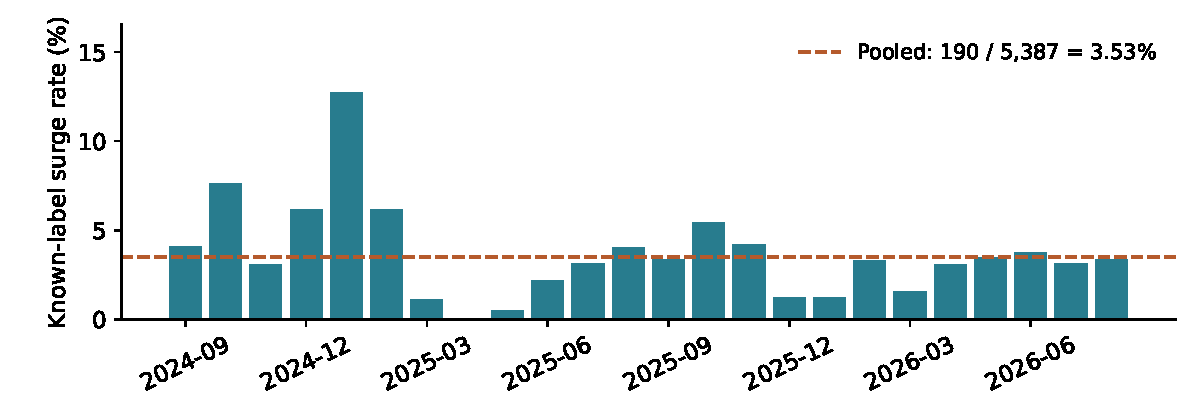
\includegraphics[width=0.80\linewidth]{figures/class_balance.pdf}\end{center}
{\small\textbf{Figure 1.} Surge share among eligible AI-maintenance article--months with known outcomes, September 2024--August 2026, original-main. 190 surges / 5,387 known rows (3.53\%); 5,197 non-surges. The unit is an article--month, not an independent article.}

One unknown outcome is excluded from 5,388 prediction-time rows. April 2025 has zero events. Available data do not support a matched full-window AI/outside-AI rate comparison.

\textbf{Recognizable product examples.} \href{https://openai.com/index/sora/}{Sora} is OpenAI's video-generation model, first shown February 15, 2024; \href{https://openai.com/index/sora-2/}{Sora 2 launched September 30, 2025}, just before the Sora article's October surge. Google's \href{https://blog.google/innovation-and-ai/technology/developers-tools/gemma-open-models/}{Gemma open-weight model family launched February 21, 2024}; \href{https://cloud.google.com/blog/products/ai-machine-learning/gemma-4-available-on-google-cloud/}{Gemma 4 followed April 2, 2026}, the month of the Gemma article's surge. This timing supplies context, not causal proof, and the measured articles remain Sora and Gemma.
\begin{center}\small
\begin{tabular}{@{}llrrr@{}}\toprule
Article & Month & Prior $I_c$ & Target $I_M$ & $T_M$\\\midrule
Sora & 2025-10 & 3,012 & 12,634 & 4,680.30\\
Gemma & 2026-04 & 362 & 2,340 & 668.81\\
\bottomrule\end{tabular}\end{center}
{\small Both meet the strict surge label and candidate filters in both original-main and Brainiac-excluded scope. Figure 1's denominator is unchanged. Counts are incoming link transitions: Sora compares 30 to 31 days, Gemma 31 to 30. Thresholds use daily-rate adjustment.}

Sora and Gemma exceeded their thresholds by 2.70 and 3.50 times, with day-adjusted increases of 305.9\% and 568.0\%.

\newpage
\sect{3. Models: what is learned and why}
\textbf{Two rule baselines.} Volume ranks the current incoming count $I_c$ and tests whether recent popularity alone is sufficient. Momentum extrapolates daily-rate growth and ranks the margin above the surge threshold:
\[
 s_{\mathrm{Momentum}}=\log(1+D_Mv_c^2/v_{c-1})-\log(1+T_M).
\]
Neither rule is trained or tuned; Momentum is not clipped.

\textbf{Logistic regression.} A linear function of the input features models the log-odds of a surge; applying the sigmoid gives an event probability. L2 regularization limits unstable coefficients. Log13 and its text-availability extension are configurations of this same algorithm.

\textbf{Histogram gradient boosting (HGB).} This classifier adds shallow decision trees to reduce binary classification loss. It tests nonlinear interactions beyond Logistic regression and outputs a surge probability.

\textbf{LightGBM classifier.} This boosted-tree probability model uses binary classification loss, month-balanced weights and the ranker's numeric inputs, testing nonlinear interactions with a fixed small tree configuration.

\textbf{Linear pairwise model with rule blend.} A linear score is learned from positive--negative article pairs within each month, encouraging a surge article to outrank a non-surge article. Its within-month percentile rank is blended with the strong threshold-margin rule's percentile rank. The output is an ordering score, not a calibrated probability. 

\textbf{Binary LambdaRank.} Boosted trees learn relative ordering with each target month as a query group. Pairs receive more weight when a swap affects top positions. Rank50 uses binary gains, truncation 50 and the rule margin as its initial score. It outputs a relative score rather than a probability, directly targeting a limited review list.

\sect{4. Features: what information predicts a surge?}
The retained ranker uses \textbf{five numeric inputs}, grouped below by meaning. All are computed before the target month. Let $L(z)=\log(1+z)$; $v_c$, $m_6$, $s_6$, $x_M$ and $T_M$ are defined in Section 2.
{\small\textbf{Table 1.} Calculation, interpretation and predictive rationale.}
\par
{\small\begin{tabularx}{\linewidth}{@{}>{\raggedright\arraybackslash}p{0.20\linewidth}>{\raggedright\arraybackslash}X@{}}\toprule
Information & Inputs and why they may help \\\midrule
Traffic scale and variability (2 inputs) & $L(v_c)$ measures current daily incoming traffic. $L(s_6)-L(m_6)$ compares historical fluctuation with typical traffic. Together they distinguish established attention from a volatile baseline, so the same increase need not imply the same risk.\\
Recent growth (2 inputs) & $L(v_c)-L(v_{c-1})$ measures month-to-month incoming growth. The pageview input is $L($mean daily views in the latest 14 days$)-L($mean in the preceding 14 days$)$. Rising navigation or recent viewing may signal attention building before a surge.\\
Distance to the surge threshold (1 input) & $L(x_M)-L(T_M)$ compares traffic projected at the current daily rate with the next month's surge threshold. A less negative value means less additional traffic is needed to cross the threshold.\\
Optional article text & Cached introductions supply topic information. SVD summarizes word patterns; LDA summarizes topics; MiniLM/PCA summarizes semantic embeddings. Each adds eight numbers plus an indicator: 1 means text unavailable, 0 means available. This distinguishes missing text from a genuine zero representation, not a missing outcome label.\\
\bottomrule\end{tabularx}}
Log13 retains its original 13 inputs, adding broader history, trend, seasonality and pageview detail from the same sources. Its full field list and the ranker's exact mapping are documented in the source package; no experimental input was removed.

\newpage
\sect{5. Preprocessing and chronological validation}
\textbf{Sources and availability.} Published Wikimedia Clickstream internal \texttt{link} edges are summed by canonical destination; published edges have counts of at least 10. Suppressed/absent article-month traffic is unknown, not zero. Pageviews supply recent attention; revisions supply the edit filter. Redirect mappings define the catalogue, without separately aggregating alias traffic. Explicit daily pageview zero is observed; a missing date is missing. Numeric features for target $M$ end at $M-1$.

\textbf{Numeric preparation.} Log13 includes current/previous log daily clickstream, three-month mean, six-month median/slope, seasonal traffic and missing flag, pageviews, 14-day growth, incomplete-PV flag, robust scale, and margins relative to $U_M$ and $T_M$. The raw slope is the intended exception to log transforms. Each fold fits imputation medians and scaling on TRAIN only; all-missing columns use zero and near-zero standard deviations use one. Logs and median/MAD summaries limit heavy-tail sensitivity. No outcome-based clipping or ad hoc extreme-surge removal is applied. Missing revision parents, hidden records or incomplete coverage imply unknown edit quality; net bytes cannot detect equal-size rewrites.

\textbf{Text preparation.} Cached text is dated at or before September 30, 2023. The availability indicator is the code field \texttt{docs[pageid]['missing']}, equal to one when no usable document is available. Missing documents receive zero semantic vectors plus this indicator; candidates are never dropped for missing text. Lexical representations use introductions and, where available in the cached source, categories. Vocabularies, SVD, LDA and PCA fit distinct usable TRAIN articles only. MiniLM remains frozen. Text is a fixed historical snapshot. The LambdaRank ablation uses the same cached documents and availability mask for every text representation.

\textbf{Time splits.} At target $M$, training uses known outcomes strictly before $M$; each row's inputs end at its own target minus one. Every preprocessing step repeats within that boundary. Selection windows precede the common September 2024--August 2026 backtest. Logistic/HGB use expanded TRAIN, including otherwise eligible high-edit rows; LightGBM/LambdaRank use candidate-eligible TRAIN. Pairwise training-pool choice is recorded below. These are comparisons of complete recipes, not isolated loss functions.

\textbf{Monthly execution.} Build candidates at the end of the completed input month, apply fold preprocessing, score all candidates and return the top 50. Future labels do not affect candidate construction. Evaluation removes unknown labels identically for all methods. Ties use current count descending, then page ID ascending. Predictions are generated for April 2025 as for every other backtest month.

\newpage
\sect{6. Hyperparameter tuning}
{\small\textbf{Table 2.} Actual search ranges, selection data and retained values. P@5 selection is preserved; it is not relabeled as NDCG@50 optimization.}
\par
\begin{tabularx}{\linewidth}{@{}>{\raggedright\arraybackslash}p{0.21\linewidth}>{\raggedright\arraybackslash}X@{}}\toprule
Algorithm & Search and choice \\\midrule
Logistic & Log13: fixed $\lambda=.01$. Numeric variants: $\lambda\in\{.001,.01,.1,1\}$ on 3 input designs (12 configurations). Text controls: $\lambda\in\{.01,.1,1\}$ on 5 input designs (15). February/May/August 2024, mean P@5 then AP; retained text-availability control uses .01.\\
HGB & Depth $\{2,3\}\times$ L2 $\{1,10\}$: 4 configurations / 12 fits on the same three months. P@5 then AP selects depth 2, L2 1.\\
LightGBM & Fixed classifier configuration below; no hyperparameter search.\\
Pairwise / rule & L2 $\{.01,.1,1\}$, expanded/candidate TRAIN, pairwise/logistic loss, weights $\{0,.1,.25,.5,1\}$: 60 scored combinations / 96 fits. January--August 2024, P@5 then AP selects pairwise, expanded TRAIN, L2 .01, learned weight .25.\\
LambdaRank & Tree parameters fixed below. Five feature designs in Table 4, January--August 2024: 40 recipe-folds (8 reused). P@50, then NDCG@50, then macro recall retains numeric inputs.\\
\bottomrule\end{tabularx}

\sect{Fixed parameters and representation controls}
\textbf{Logistic.} The objective is mean binary cross-entropy plus $\lambda\|\beta\|^2/2$, with an unpenalized intercept. Damped Newton has a 200-step cap and gradient tolerance $10^{-9}$. Log13 uses its inherited fixed value.

\textbf{HGB.} Fixed settings are 100 boosting iterations, learning rate .05, 32 bins, $2^{\mathrm{depth}}$ leaves and minimum leaf size $\max(30,\lceil .05n\rceil)$. No early stopping or class weighting is used. The bounded depth/L2 search tests capacity without a large grid.

\textbf{LightGBM and LambdaRank.} Both fix 100 trees, 7 leaves, depth 3, learning rate .03, L2 10, minimum leaf 30, 63 bins, seed 718, and full row/feature fractions. The threshold-margin coefficient is monotone positive. The classifier balances months; the ranker groups rows by month with binary gains and truncation 50. There is no early stopping or subsampling. The initialized ranker's standardized rule margin is added exactly once at prediction. Fixed shallow trees limit capacity with sparse positives.

\textbf{Pairwise and blend.} Each month has equal weight, with up to 200 negatives per positive (seed 718). L-BFGS-B uses 500 iterations, gradient tolerance $10^{-7}$ and function tolerance $10^{-12}$. Blending combines within-month percentile ranks rather than probabilities.

\textbf{Feature controls, not additional algorithms.} Numeric Logistic tuning also compared the original slope, signed-log slope and five added dynamics. Text controls compared the availability indicator alone with lexical SVD, LDA, category SVD and MiniLM/PCA additions. The main table reports reference Logistic and the availability-only configuration; Table 4 holds LambdaRank fixed.

Lexical features use English stopwords, unigrams, minimum document frequency 2, maximum fraction .95 and at most 3,000 terms. SVD fixes 8 dimensions and 7 power iterations; LDA fixes 8 topics and 20 iterations; PCA fixes 8 components with the full solver. MiniLM uses \texttt{all-MiniLM-L6-v2} from \texttt{sentence-transformers}, revision \nolinkurl{7dbbc90392e2f80f3d3c277d6e90027e55de9125} (2022), with normalized 384-dimensional vectors and a 256-wordpiece limit. Dimensions and seeds were fixed.

\newpage
\sect{7. Fair comparison on common development support}
{\small\textbf{Table 3.} Original-main only: the same 24 months, 5,387 known candidate rows, 190 events and 1,200 review slots for every row. All values are reaggregated from saved monthly results.}
\begin{center}\small
\begin{tabular}{@{}llrrrr@{}}\toprule
Algorithm & Features / configuration & NDCG@50 & P@50 & Recall@50 & AP\\\midrule
Volume & Current count & 0.1235 & 0.0392 & 0.2474 & 0.0615 \\
Momentum & Growth margin & 0.2412 & 0.0633 & 0.4000 & 0.1122 \\
Logistic & Log13 reference & 0.2651 & 0.0675 & 0.4263 & 0.1284 \\
Logistic & Log13 + text availability & 0.2741 & 0.0733 & 0.4632 & 0.1323 \\
HGB & Numeric + dynamics & 0.2408 & 0.0667 & 0.4211 & 0.1060 \\
LightGBM & Compact numeric & 0.2777 & 0.0650 & 0.4105 & 0.1365 \\
Linear pairwise & Compact numeric + rule blend & 0.2819 & 0.0675 & 0.4263 & 0.1417 \\
LambdaRank & Compact numeric, Rank50 & 0.2965 & 0.0733 & 0.4632 & 0.1458 \\

\bottomrule\end{tabular}\end{center}

For month $m$ with $E_m$ events, binary $\mathrm{DCG}_{50}=\sum_{r=1}^{50}y_r/\log_2(r+1)$ and NDCG divides this by the ideal DCG on the same candidate pool. \textbf{NDCG and full-list AP average the 23 event months equally}. P@50 averages all 24 months and equals pooled hits/1,200. \textbf{Recall here is pooled}: $\sum_m\mathrm{TP}_{50,m}/\sum_mE_m$, retaining the original submission's aggregation. Macro recall is a different statistic (equal weight per event month) and is not substituted silently. April 2025 was predicted and evaluated: precision is zero, while NDCG/AP/recall are undefined because there are no positive labels. Ties use current count descending, then page ID ascending.

Numeric Rank50 adds 12 hits over Momentum (88 versus 76): about 3.67 versus 3.17 hits per 50-item monthly list. The remaining reviewed items are non-events under this traffic definition, so absolute precision is still low. Against Log13 it adds seven hits, but macro recall is slightly lower (0.4955 versus 0.4998), illustrating a monthly weighting tradeoff.

\begin{center}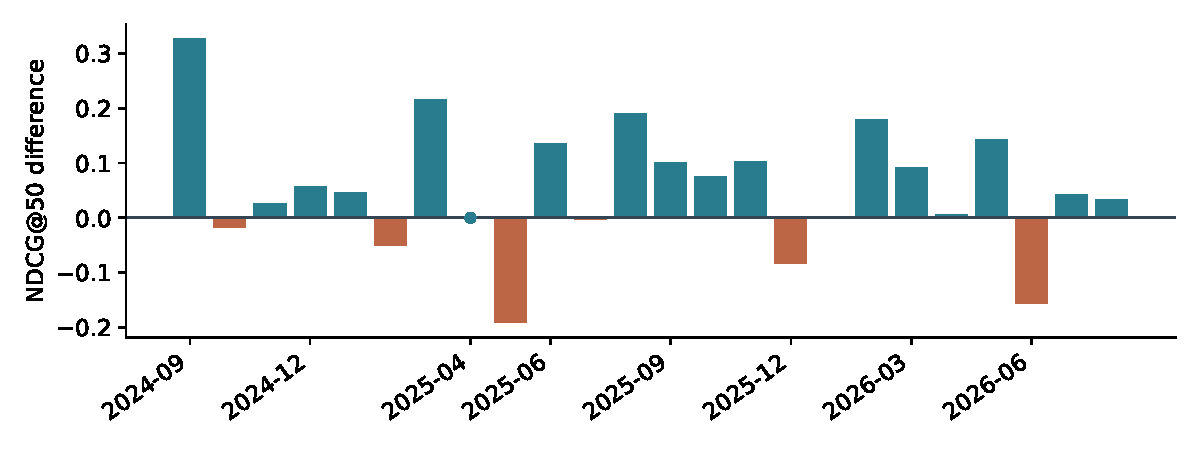
\includegraphics[width=\linewidth]{figures/monthly_delta.pdf}\end{center}
{\small\textbf{Figure 2.} Numeric Rank50 minus Momentum in binary NDCG@50, by month, on original-main. A positive average does not imply uniform improvement. For plotting only, the zero-event month (April 2025) is shown at zero; aggregate NDCG averages event months.}

\src{\texttt{user\_at50\_history\_v1/summary.csv} and \texttt{monthly.csv}; equal-support assertions and independent aggregation in the source bundle.}

\newpage
\sect{8. Does article text improve ranking?}
All five rows use the \textbf{same LambdaRank learner, training splits and parameters}. Only the added input changes. Each row is a separate comparison with numeric-only, not a sequence of cumulative additions. The three content representations each include the same text-availability flag; the control uses that flag alone.

{\small\textbf{Table 4.} Added text information on the common development backtest.}
\begin{center}
\begin{tabular}{@{}lrr@{}}\toprule
Added information & NDCG@50 & $\Delta$ vs numeric-only\\\midrule
None (numeric only) & 0.2965 & +0.0000 \\
Text availability only (control) & 0.2929 & -0.0036 \\
Word patterns (TF-IDF / SVD) & 0.3086 & +0.0121 \\
Topic mixture (LDA) & 0.2676 & -0.0289 \\
Semantic meaning (MiniLM / PCA) & 0.2882 & -0.0083 \\

\bottomrule\end{tabular}\end{center}

Word-pattern features improve NDCG@50 over both numeric-only and the availability-only control; topic and semantic features do not exceed numeric-only. Thus text coverage alone does not explain the word-pattern improvement. The earlier P@50-selected numeric model remains retained: the highest development score is not used to select a replacement.

\sect{9. Discussion and robustness}
\textbf{Failures remain evidence.} The pairwise blend also made harmful Top5 exchanges in development: one added event versus five removed. Better @50 NDCG therefore cannot justify a claim that every operational budget improved. Numeric Rank50 loses NDCG@50 to Momentum in 7 of 23 event months and wins in 16. The largest losses are May 2025 ($-0.1920$), June 2026 ($-0.1557$) and December 2025 ($-0.0827$).

\textbf{Separate clean sensitivity.} Excluding Brainiac from both sides leaves 5,382 known rows, 189 events and 24 months (23 with events). Saved clean NDCG@50/P@50 are Volume .1237/.0392, Momentum .2418/.0633, Log13 .2638/.0667 and binary numeric Rank50 .2893/.0742. Rank50 finds 89 events, pooled recall $89/189=.4709$, versus Momentum's $76/189=.4021$. This preserves a positive point difference, but clean results are unavailable for every displayed family. They are \textbf{not mixed into Table 3}, and exclusion is a sensitivity analysis, not a complete historical-identity repair.

\textbf{Version change.} The previously submitted PDF used 23 scored months, 182 events and 1,150 slots. This report uses the later 24-month original-main records and recomputes all displayed baselines under the same support and metric definitions. Differences across those reports must not be interpreted solely as model improvement.

\src{Model and input selection records; separate clean values from the separate clean-summary record.}

\newpage
\sect{10. Interpretation and reproducibility}
\textbf{Operational interpretation.} The retained numeric binary Rank50 recipe improves average early ranking and total event capture relative to Momentum on the common development backtest. Its 88 hits represent 46.32\% pooled recall at a 50-item monthly budget. Yet low precision and month-specific losses mean an automated shortlist should assist human review rather than trigger automatic edits. Surge detection is only a proxy for where a review may be useful; it does not measure article quality or the value of a resulting edit.

\textbf{Generalization limits.} The 24 reported months and early selection windows have been examined repeatedly during model development. The results therefore describe development performance, not an independent test. The sealed September 2026 holdout remains unevaluated. Historical source-release availability, catalogue hindsight and title identity remain limitations of deployment realism. The separate clean sensitivity supports the direction of the numeric ranker's average comparison, but does not certify all historical identities or provide clean results for every family.

\textbf{Continuous exploration.} Earlier continuous-target experiments include regression and graded ranking of relative traffic excess. They use different losses and selection metrics. This report focuses on the binary task and does not use continuous-model results to select its binary recipe.

\sect{Reproducibility and evidence}
The companion source package contains \texttt{main.tex}, vector PDF figures, generated table rows, selected monthly/aggregate CSV records, source SHA256 hashes and a zero-fit aggregation script. Compile with \texttt{tectonic main.tex}. The provided table/figure assets make PDF compilation independent of the local data workspace. Regenerating the figures uses saved development CSVs and performs no model training.

The report-aligned code and reproduction instructions are in \href{https://github.com/Lyleeeeeeee/10718_MLinPractice/tree/main/wikiflow/binary}{the dedicated binary submission directory}. It preserves the original development data contract and adds only the methods and evidence discussed here.

The current comparison draws from \texttt{research/results/user\_at50\_history\_v1/} and selection metadata in \texttt{task\_views\_history\_v1/}, with the corresponding fixed configurations and selection records linked in the source mapping. The accompanying selected CSVs reproduce every displayed aggregate; full trial records remain in the project. The clean sensitivity uses the separate clean-summary record. All new report outputs were generated separately from experimental inputs.

\textbf{Course context.} The report addresses the metric-choice and baseline-results feedback verified October 20, and the \href{https://canvas.cmu.edu/courses/56403/assignments/1023752}{Initial ML Solution requirements}: task/population and budget, temporal validation, preprocessing, family rationale/tuning, comparable baselines, and adverse results. \href{https://docs.google.com/spreadsheets/d/1QIaExyCzQZRZ8s9_8-jXQsVivJHy3t5D_VwVCl5kEWs/edit#gid=1437791232}{Prior feedback} motivates the explicit metric revision and common-support comparison.
\end{document}
